
\usepackage{tikz} 
\usepackage{mathptmx}
%\usepackage[T1]{fontenc}
\usepackage[latin1]{inputenc}
\usepackage{color}
\usepackage{amsmath}
\usepackage{amssymb}


%%%%%%%%%% Farseerfc: fix the bug of xetex on navigation bar of beamer %%%%%%%%%

\def\beamer@linkspace#1{%
  \begin{pgfpicture}{0pt}{-1.5pt}{#1}{5.5pt}
    \pgfsetfillopacity{0}
    \pgftext[x=0pt,y=-1.5pt]{.}
    \pgftext[x=#1,y=5.5pt]{.}
  \end{pgfpicture}}

%%%%%%%%%% Farseerfc: fix the bug of xetex on navigation bar of beamer %%%%%%%%%

\usetheme{Warsaw}
\usecolortheme[named=OliveGreen]{structure}
%\setbeamercovered{dynamic}
\useoutertheme{infolines}
\usepackage[english]{babel}


\graphicspath{{figure/}}
\begin{document}

%%%%%%%%%%%%%%%%%%%%%%%%%%%%%%%%%%%%%%%%%%%%%%%%%%%%%%%%%%%%%%%%%%%%%%%%%%%%%%%%
% Farseerfc defined commands

\newcommand{\br}[0]{\par\vskip15pt\par}
%\newenvironment{topcolumns}{\begin{columns}[t]}{\end{columns}}

%%%%%%%%%%%%%%%%%%%%%%%%%%%%%%%%%%%%%%%%%%%%%%%%%%%%%%%%%%%%%%%%%%%%%%%%%%%%%%%%



\title[SuffixTree]{Algorithm of Suffix Tree Construction}

\subtitle{by farseerfc@gmail.com}

\author[jc-yang]{
	Jiachen Yang\inst{1} 
}

\institute[Osaka-U]{
	\inst{1}Research Student in Osaka University
}



\frame{\maketitle}


\AtBeginSubsection[]{
  \frame<beamer>{ 
    \frametitle{Section Outline}   
    \tableofcontents[currentsection,currentsubsection] 
  }
}

\AtBeginSection[]{
  \frame<beamer>{ 
    \frametitle{Part Outline}   
    \tableofcontents[currentpart,currentsection] 
  }
}

\AtBeginPart{
  \frame<beamer>{
	\partpage
  }
}

%%%%%%%%%%%%%%%%%%%%%%%%%%%%%%%%%%%%%%%%%%%%%%%%%%%%%%%%%%%%%%%%%%%%%%%%%%%%%%%%
\section{What I did} 

\begin{frame}{Algorithm of Constructing Suffix Tree}%
\begin{columns}%
\transfade[duration=0.2]<2->
\column{0.5\textwidth}
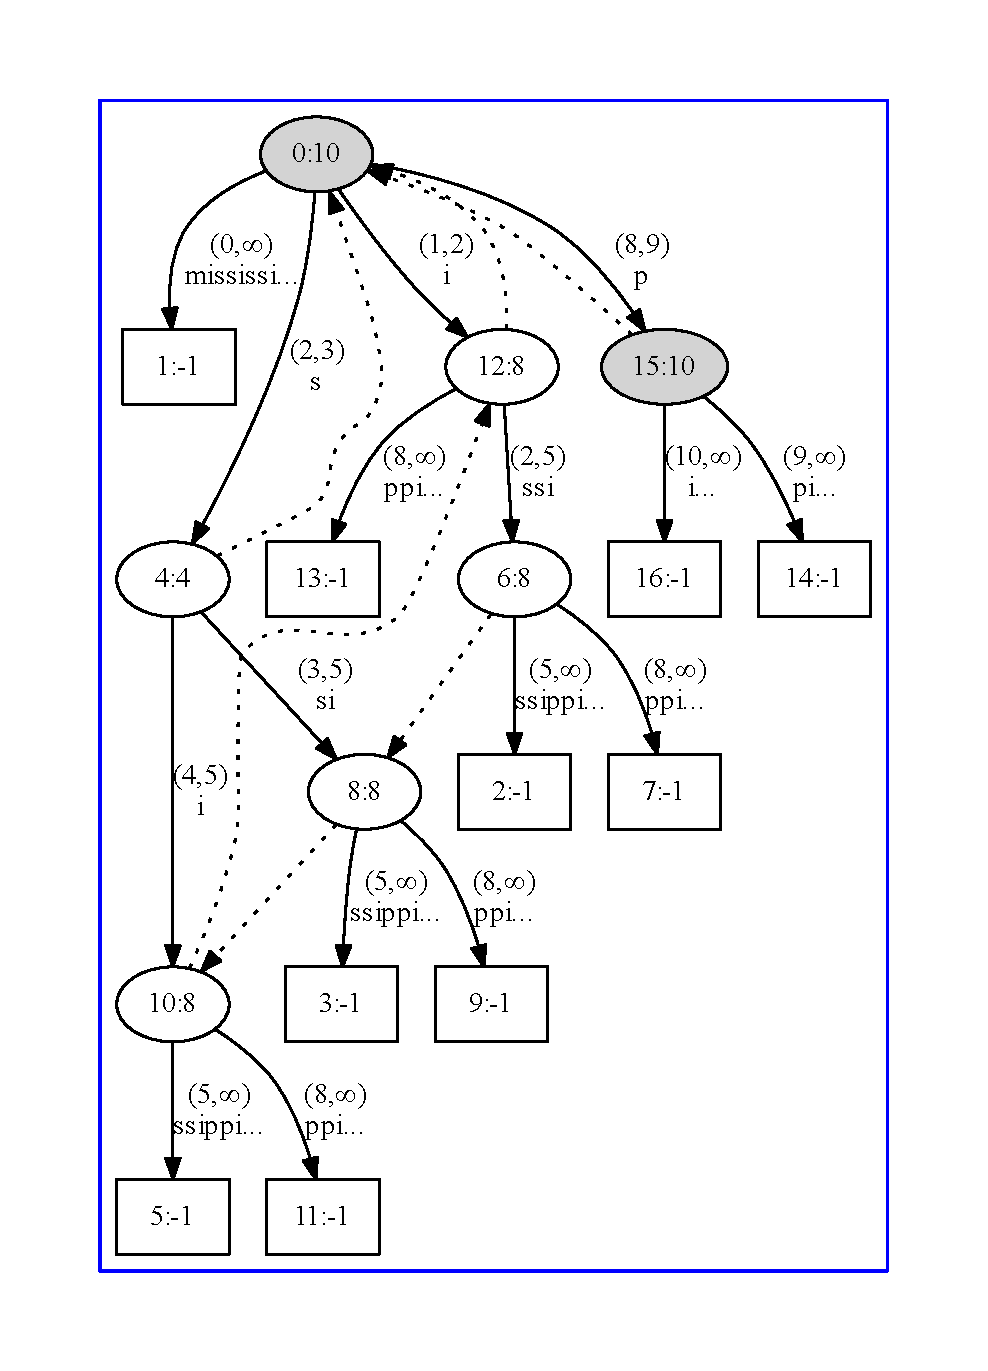
\includegraphics[width=\textwidth]{mississippi.pdf}

\column{0.45\textwidth}
\begin{itemize}
\item<2-> 
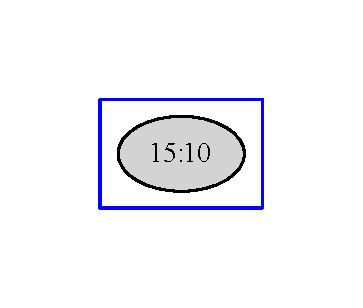
\includegraphics[width=0.25\textwidth,trim=40pt 40pt 40pt 40pt]{gray.pdf} 
Node (id:generation)
\item<3-> 
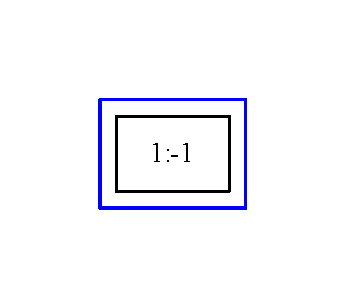
\includegraphics[width=0.25\textwidth,trim=40pt 40pt 40pt 40pt]{box.pdf} 
Leaf
\item<4-> 
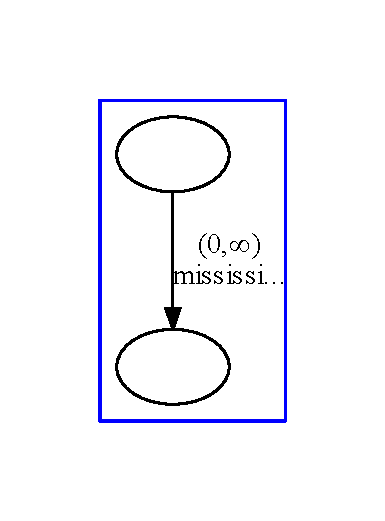
\includegraphics[width=0.25\textwidth,trim=40pt 40pt 40pt 40pt]{line.pdf} 
Child-relation
\item<5-> 
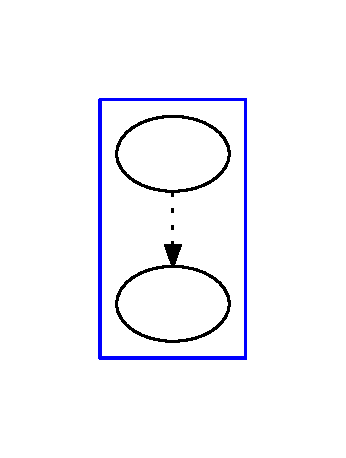
\includegraphics[width=0.25\textwidth,trim=40pt 40pt 40pt 40pt]{dotted.pdf} 
suffix-link relation
\end{itemize}
\end{columns}
\end{frame}

%%%%%%%%%%%%%%%%%%%%%%%%%%%%%%%%%%%%%%%%%%%%%%%%%%%%%%%%%%%%%%%%%%%%%%%%%%%%%%%%
\begin{frame}{Experiment -- mississippi}

\transfade[duration=0.1]<2->
\begin{overlayarea}{\textwidth}{\textheight}
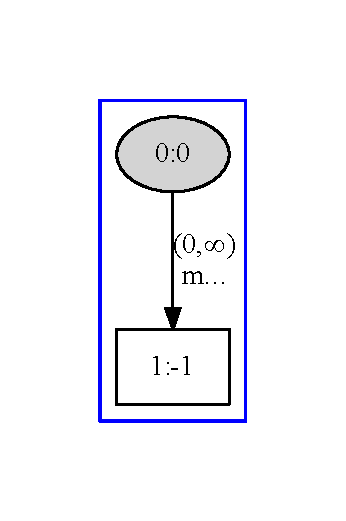
\includegraphics[keepaspectratio,height=0.9\textheight,width=0.9\textwidth]{m.pdf}<1>
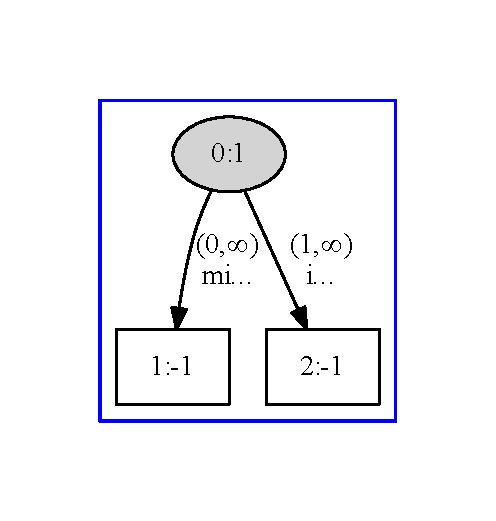
\includegraphics[keepaspectratio,height=0.9\textheight,width=0.9\textwidth]{mi.pdf}<2>
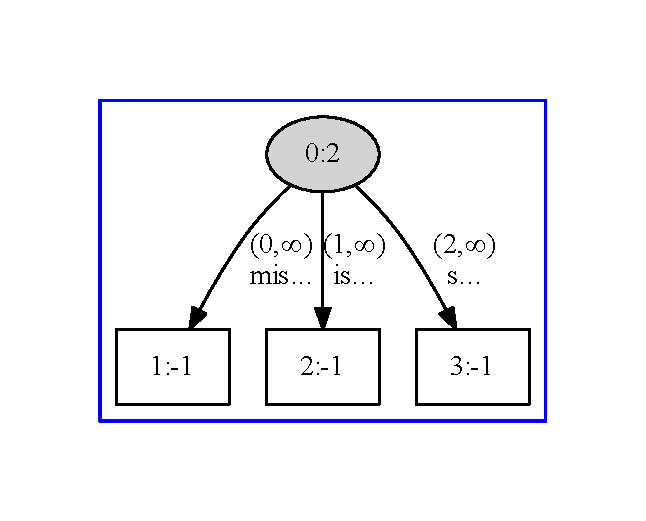
\includegraphics[keepaspectratio,height=0.9\textheight,width=0.9\textwidth]{mis.pdf}<3>
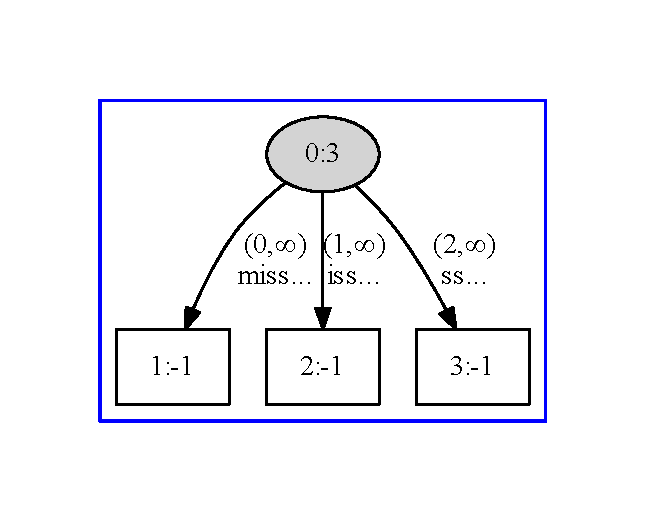
\includegraphics[keepaspectratio,height=0.9\textheight,width=0.9\textwidth]{miss.pdf}<4>
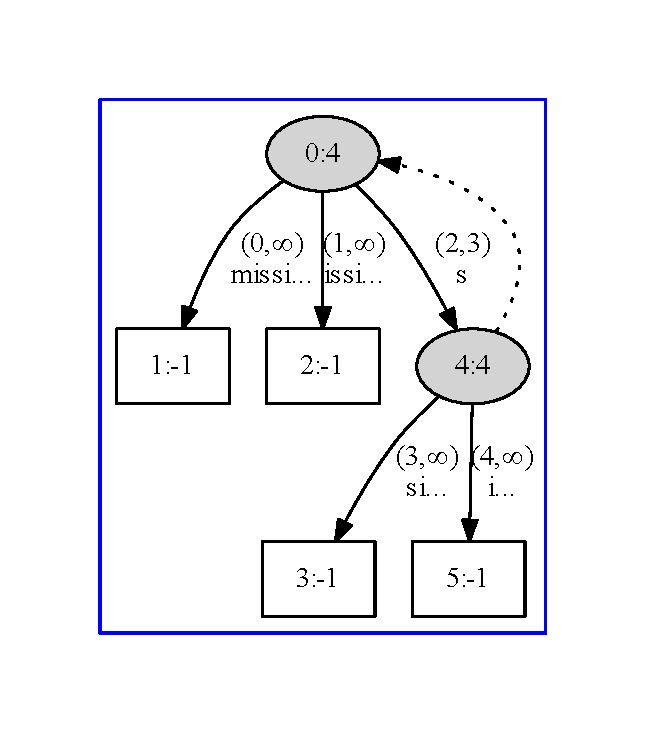
\includegraphics[keepaspectratio,height=0.9\textheight,width=0.9\textwidth]{missi.pdf}<5>
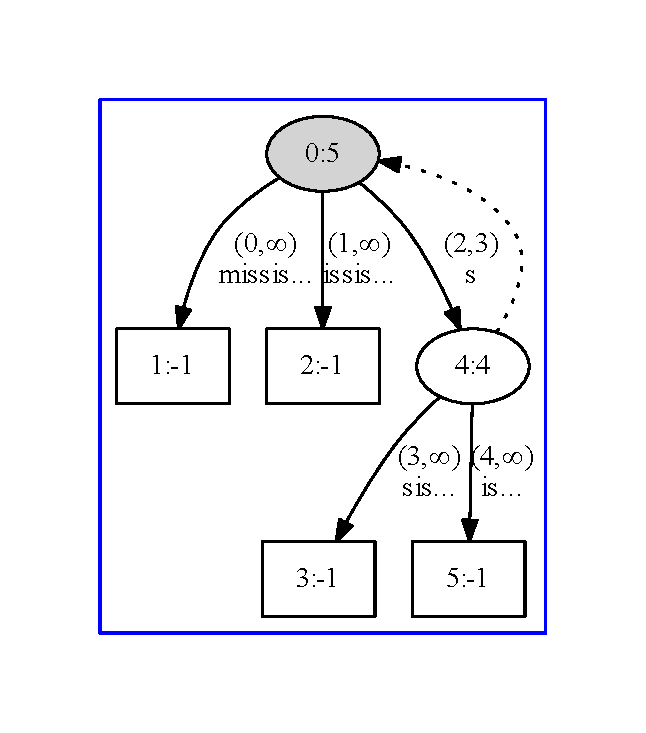
\includegraphics[keepaspectratio,height=0.9\textheight,width=0.9\textwidth]{missis.pdf}<6>
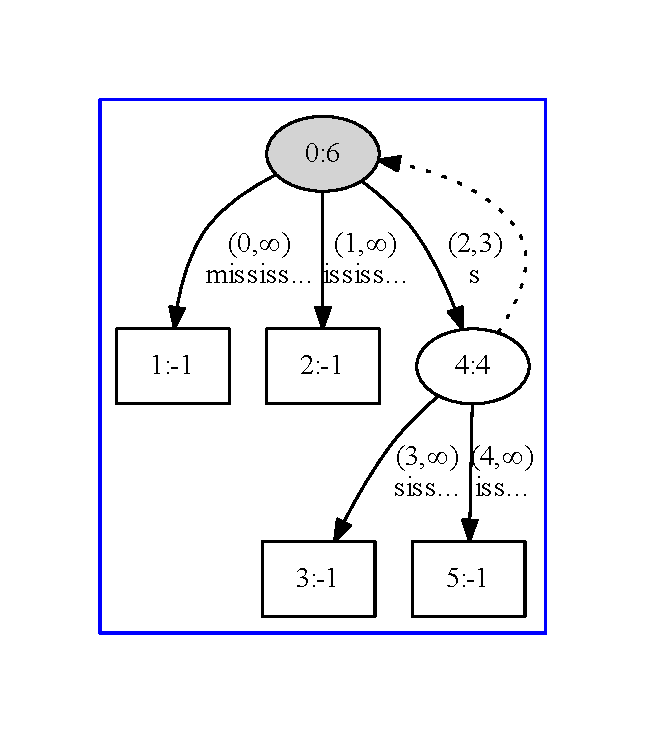
\includegraphics[keepaspectratio,height=0.9\textheight,width=0.9\textwidth]{mississ.pdf}<7>
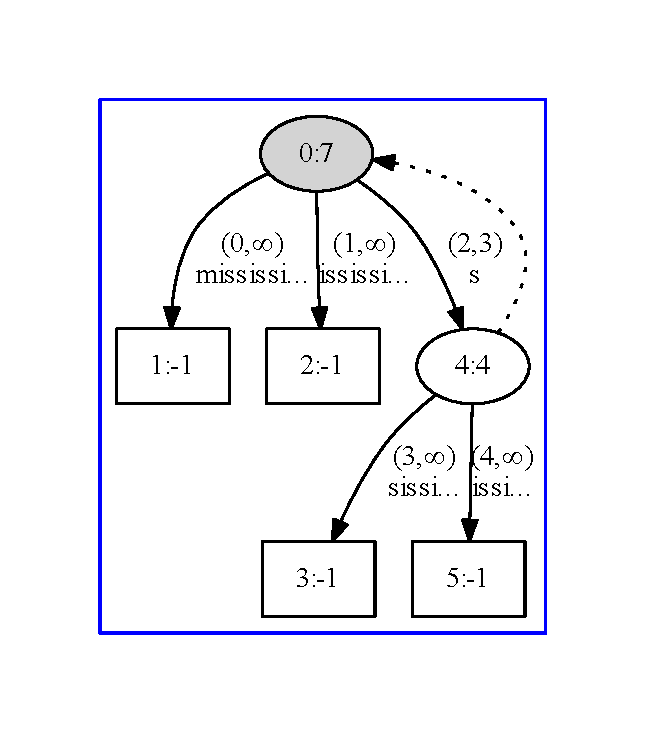
\includegraphics[keepaspectratio,height=0.9\textheight,width=0.9\textwidth]{mississi.pdf}<8>
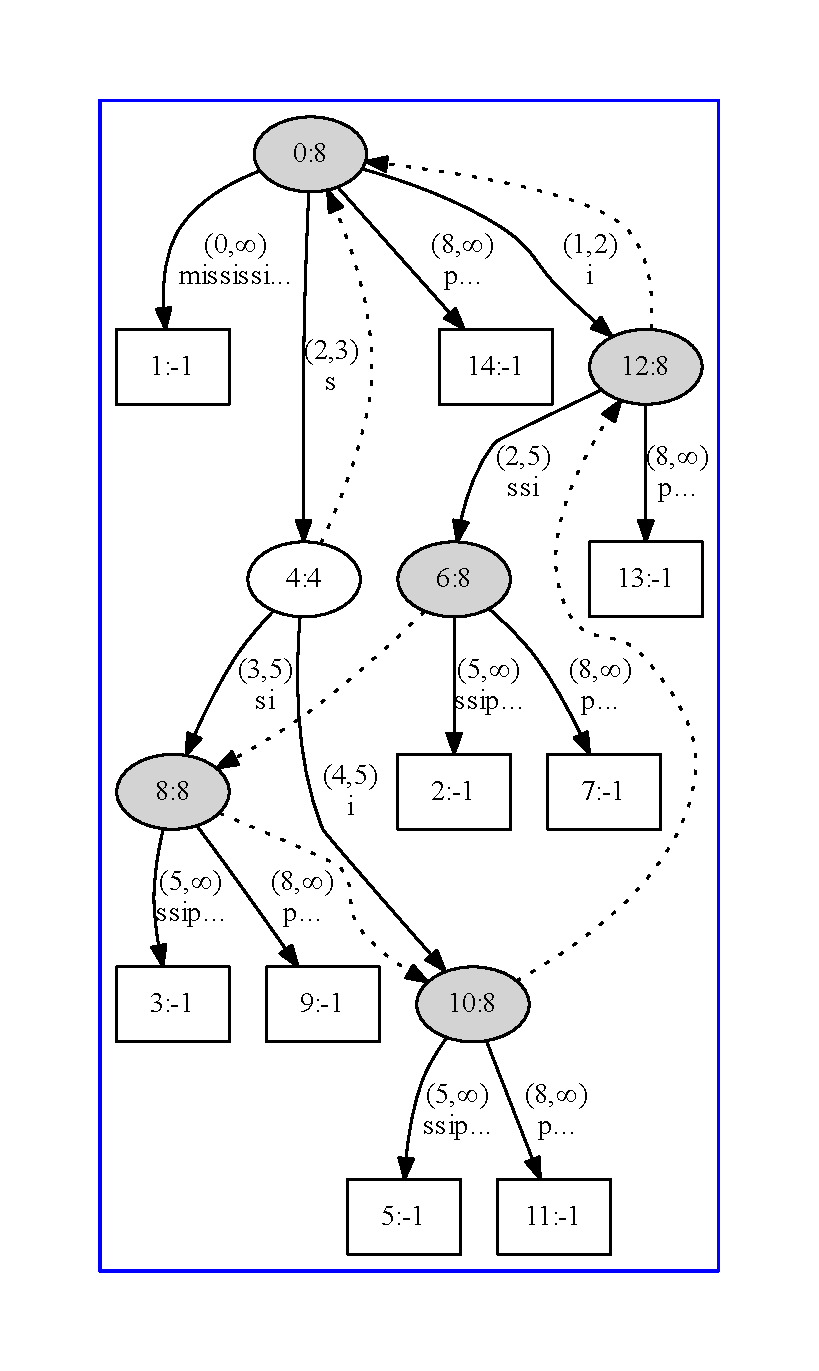
\includegraphics[keepaspectratio,height=0.9\textheight,width=0.9\textwidth]{mississip.pdf}<9>
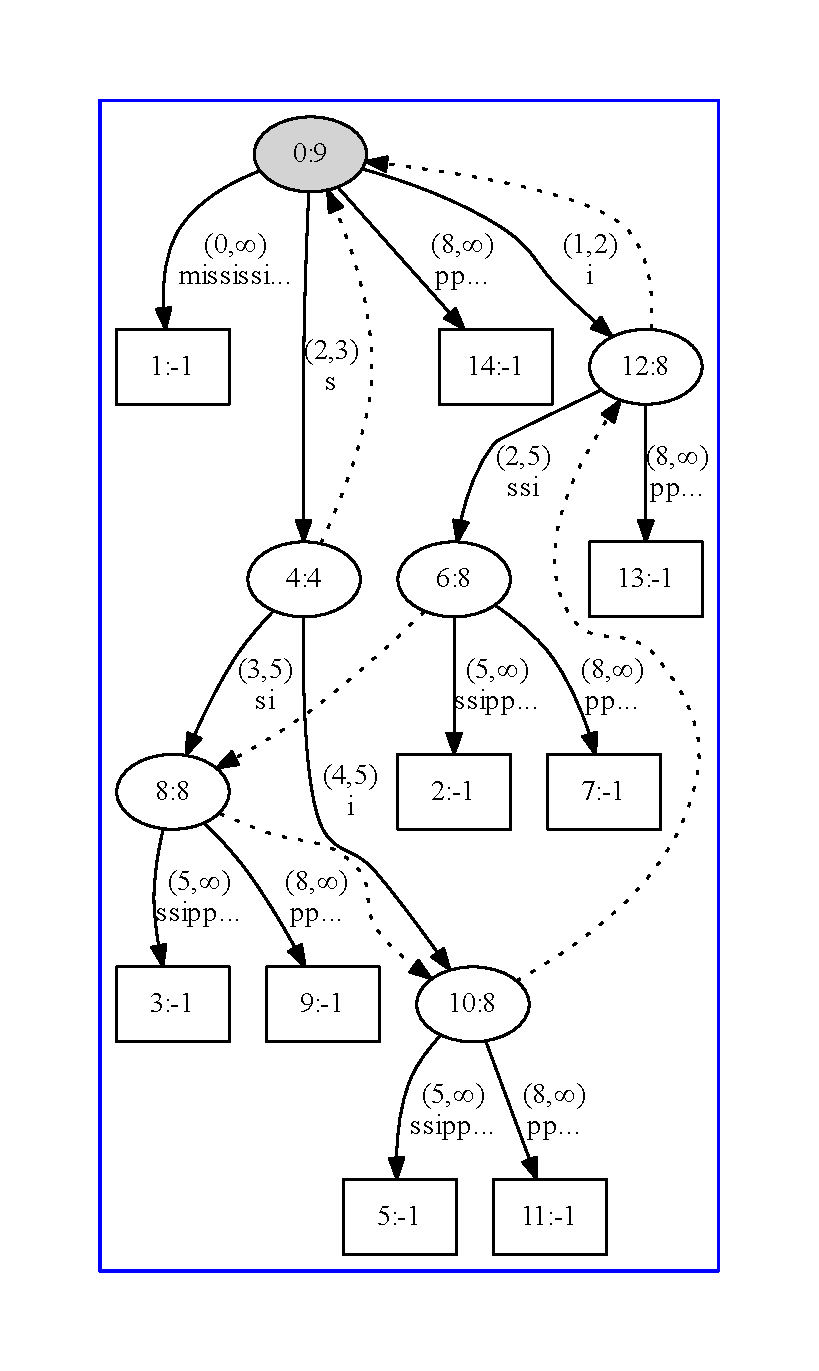
\includegraphics[keepaspectratio,height=0.9\textheight,width=0.9\textwidth]{mississipp.pdf}<10>
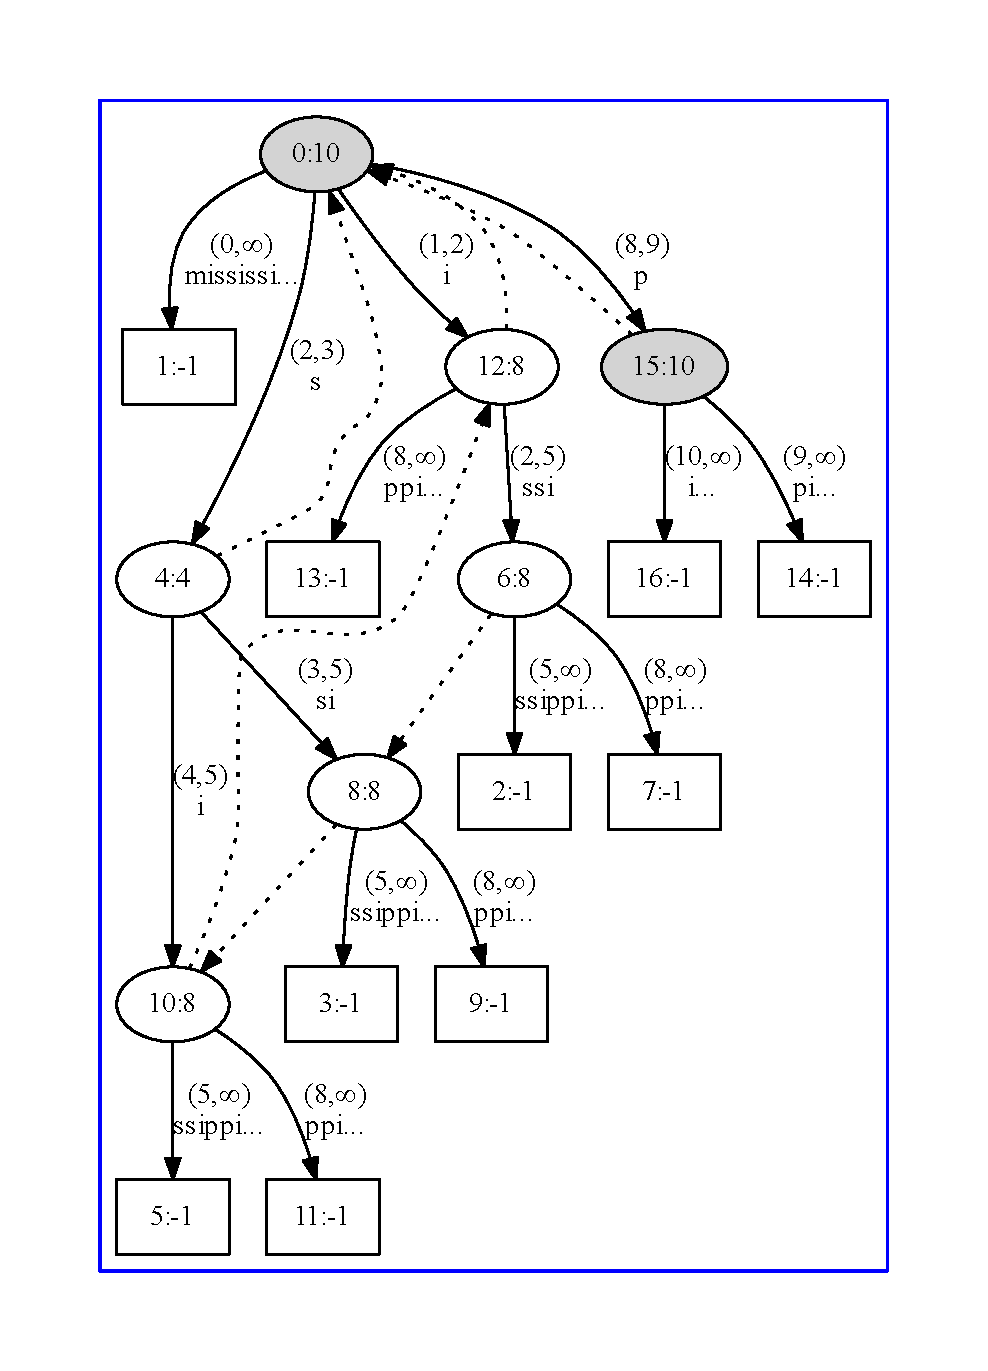
\includegraphics[keepaspectratio,height=0.9\textheight,width=0.9\textwidth]{mississippi.pdf}<11>
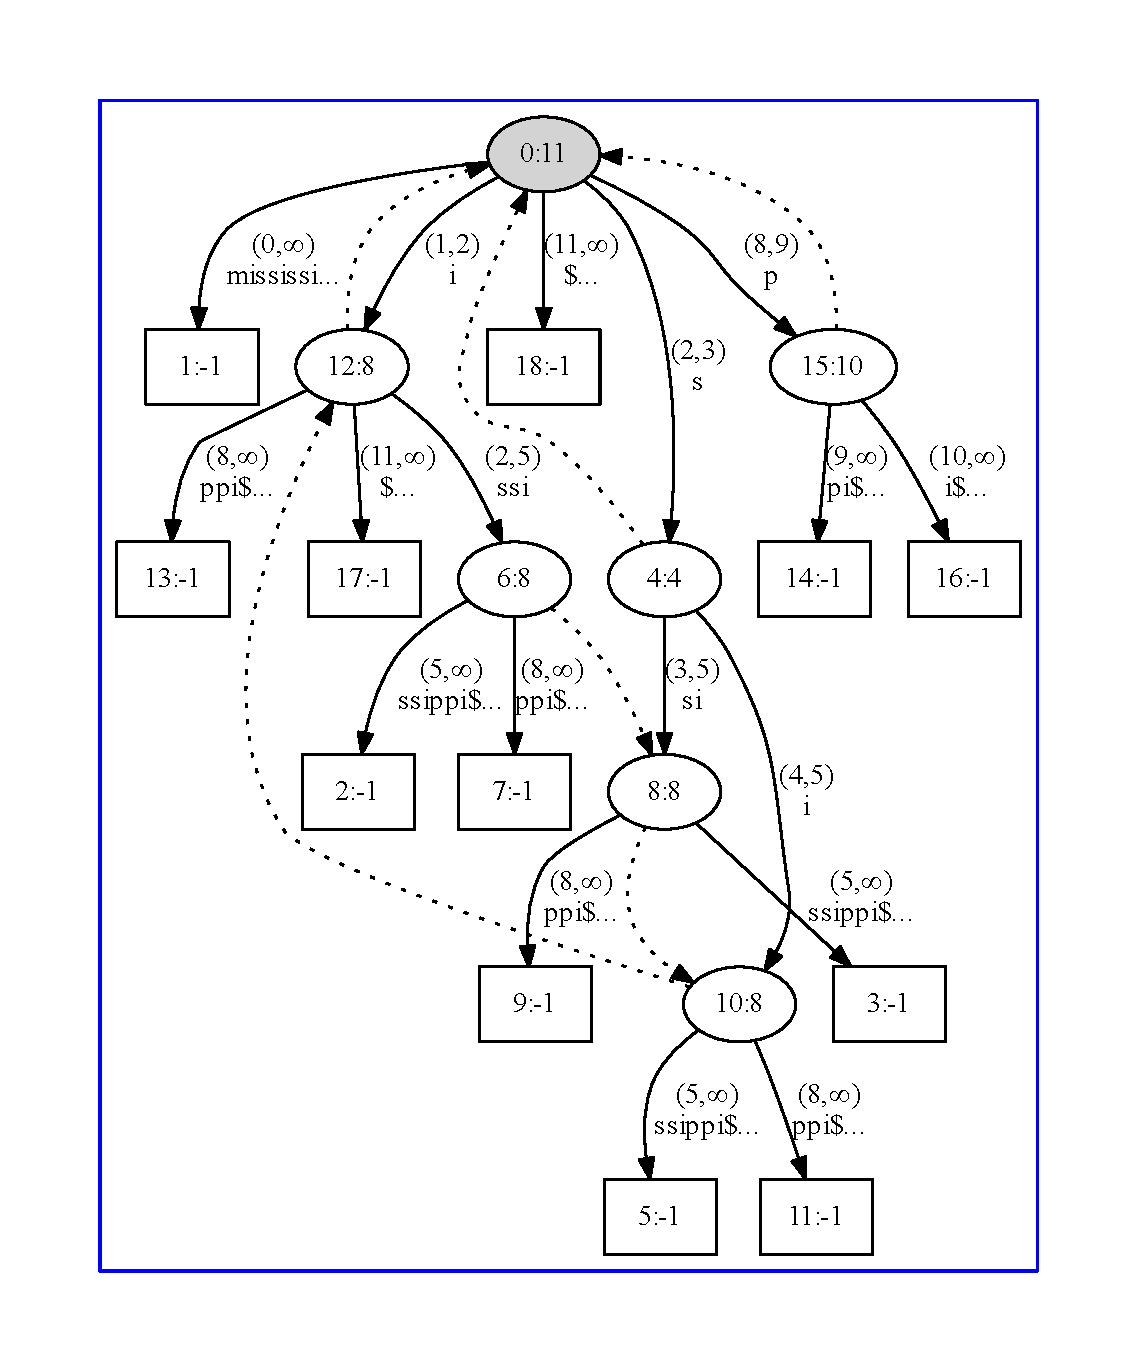
\includegraphics[keepaspectratio,height=0.9\textheight,width=0.9\textwidth]{mississippi_.pdf}<12>
\end{overlayarea}
\end{frame}
%%%%%%%%%%%%%%%%%%%%%%%%%%%%%%%%%%%%%%%%%%%%%%%%%%%%%%%%%%%%%%%%%%%%%%%%%%%%%%%%
\begin{frame}[shrink=15]{Experiment -- English text}

%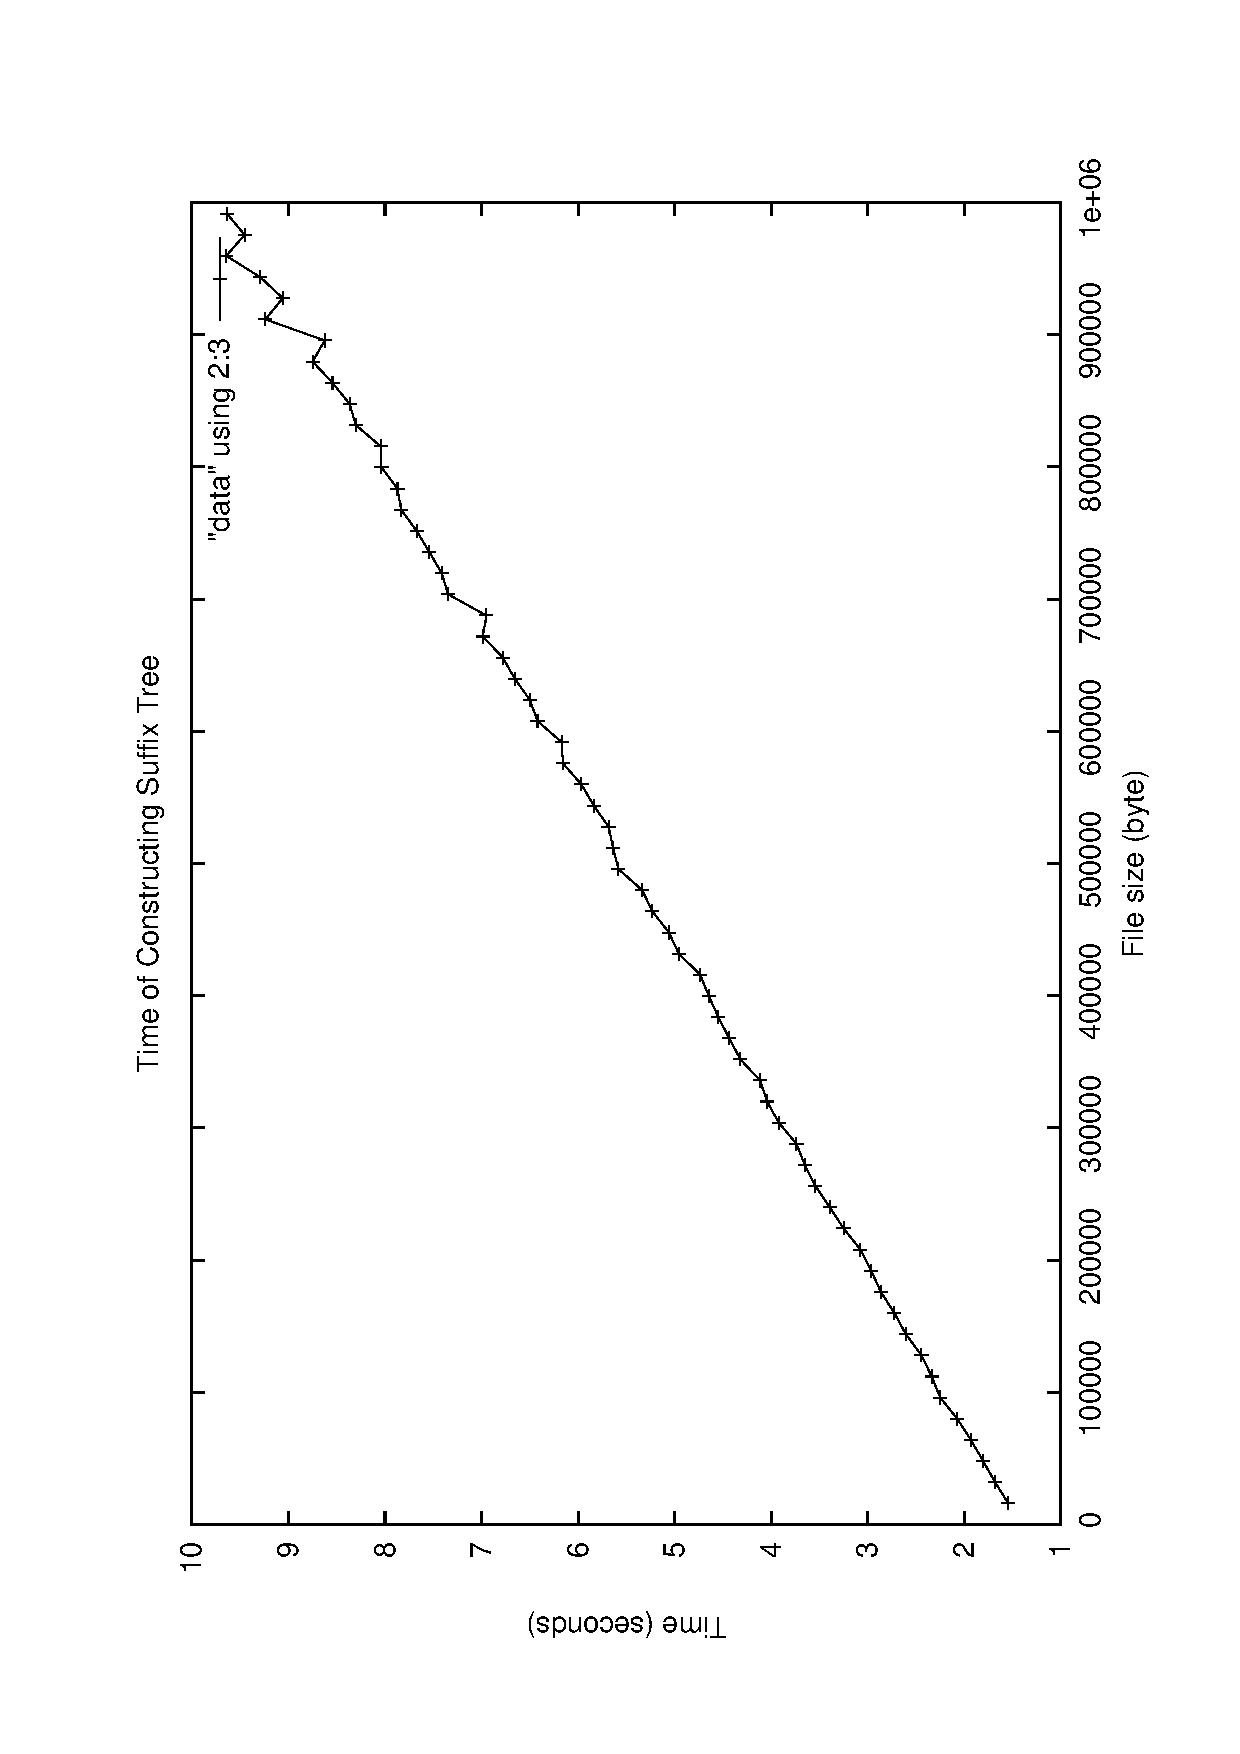
\includegraphics[angle=270,width=0.9\textwidth]{plot.fig}
%\documentclass{article}
%\usepackage{graphicx}

%\begin{document}
% GNUPLOT: LaTeX picture with Postscript
\begingroup
  \makeatletter
  \providecommand\color[2][]{%
    \GenericError{(gnuplot) \space\space\space\@spaces}{%
      Package color not loaded in conjunction with
      terminal option `colourtext'%
    }{See the gnuplot documentation for explanation.%
    }{Either use 'blacktext' in gnuplot or load the package
      color.sty in LaTeX.}%
    \renewcommand\color[2][]{}%
  }%
  \providecommand\includegraphics[2][]{%
    \GenericError{(gnuplot) \space\space\space\@spaces}{%
      Package graphicx or graphics not loaded%
    }{See the gnuplot documentation for explanation.%
    }{The gnuplot epslatex terminal needs graphicx.sty or graphics.sty.}%
    \renewcommand\includegraphics[2][]{}%
  }%
  \providecommand\rotatebox[2]{#2}%
  \@ifundefined{ifGPcolor}{%
    \newif\ifGPcolor
    \GPcolorfalse
  }{}%
  \@ifundefined{ifGPblacktext}{%
    \newif\ifGPblacktext
    \GPblacktexttrue
  }{}%
  % define a \g@addto@macro without @ in the name:
  \let\gplgaddtomacro\g@addto@macro
  % define empty templates for all commands taking text:
  \gdef\gplbacktext{}%
  \gdef\gplfronttext{}%
  \makeatother
  \ifGPblacktext
    % no textcolor at all
    \def\colorrgb#1{}%
    \def\colorgray#1{}%
  \else
    % gray or color?
    \ifGPcolor
      \def\colorrgb#1{\color[rgb]{#1}}%
      \def\colorgray#1{\color[gray]{#1}}%
      \expandafter\def\csname LTw\endcsname{\color{white}}%
      \expandafter\def\csname LTb\endcsname{\color{black}}%
      \expandafter\def\csname LTa\endcsname{\color{black}}%
      \expandafter\def\csname LT0\endcsname{\color[rgb]{1,0,0}}%
      \expandafter\def\csname LT1\endcsname{\color[rgb]{0,1,0}}%
      \expandafter\def\csname LT2\endcsname{\color[rgb]{0,0,1}}%
      \expandafter\def\csname LT3\endcsname{\color[rgb]{1,0,1}}%
      \expandafter\def\csname LT4\endcsname{\color[rgb]{0,1,1}}%
      \expandafter\def\csname LT5\endcsname{\color[rgb]{1,1,0}}%
      \expandafter\def\csname LT6\endcsname{\color[rgb]{0,0,0}}%
      \expandafter\def\csname LT7\endcsname{\color[rgb]{1,0.3,0}}%
      \expandafter\def\csname LT8\endcsname{\color[rgb]{0.5,0.5,0.5}}%
    \else
      % gray
      \def\colorrgb#1{\color{black}}%
      \def\colorgray#1{\color[gray]{#1}}%
      \expandafter\def\csname LTw\endcsname{\color{white}}%
      \expandafter\def\csname LTb\endcsname{\color{black}}%
      \expandafter\def\csname LTa\endcsname{\color{black}}%
      \expandafter\def\csname LT0\endcsname{\color{black}}%
      \expandafter\def\csname LT1\endcsname{\color{black}}%
      \expandafter\def\csname LT2\endcsname{\color{black}}%
      \expandafter\def\csname LT3\endcsname{\color{black}}%
      \expandafter\def\csname LT4\endcsname{\color{black}}%
      \expandafter\def\csname LT5\endcsname{\color{black}}%
      \expandafter\def\csname LT6\endcsname{\color{black}}%
      \expandafter\def\csname LT7\endcsname{\color{black}}%
      \expandafter\def\csname LT8\endcsname{\color{black}}%
    \fi
  \fi
  \setlength{\unitlength}{0.0500bp}%
  \begin{picture}(7200.00,5040.00)%
    \gplgaddtomacro\gplbacktext{%
      \csname LTb\endcsname%
      \put(814,704){\makebox(0,0)[r]{\strut{} 0}}%
      \put(814,1213){\makebox(0,0)[r]{\strut{} 2}}%
      \put(814,1722){\makebox(0,0)[r]{\strut{} 4}}%
      \put(814,2231){\makebox(0,0)[r]{\strut{} 6}}%
      \put(814,2740){\makebox(0,0)[r]{\strut{} 8}}%
      \put(814,3248){\makebox(0,0)[r]{\strut{} 10}}%
      \put(814,3757){\makebox(0,0)[r]{\strut{} 12}}%
      \put(814,4266){\makebox(0,0)[r]{\strut{} 14}}%
      \put(814,4775){\makebox(0,0)[r]{\strut{} 16}}%
      \put(946,484){\makebox(0,0){\strut{} 0}}%
      \put(1783,484){\makebox(0,0){\strut{} 20000}}%
      \put(2619,484){\makebox(0,0){\strut{} 40000}}%
      \put(3456,484){\makebox(0,0){\strut{} 60000}}%
      \put(4293,484){\makebox(0,0){\strut{} 80000}}%
      \put(5130,484){\makebox(0,0){\strut{} 100000}}%
      \put(5966,484){\makebox(0,0){\strut{} 120000}}%
      \put(6803,484){\makebox(0,0){\strut{} 140000}}%
      \put(176,2739){\rotatebox{-270}{\makebox(0,0){\strut{}Construction Time (sec.)}}}%
      \put(3874,154){\makebox(0,0){\strut{}File size (byte)}}%
    }%
    \gplgaddtomacro\gplfronttext{%
      \csname LTb\endcsname%
      \put(5816,4602){\makebox(0,0)[r]{\strut{}"data" using 1:3}}%
    }%
    \gplbacktext
    \put(0,0){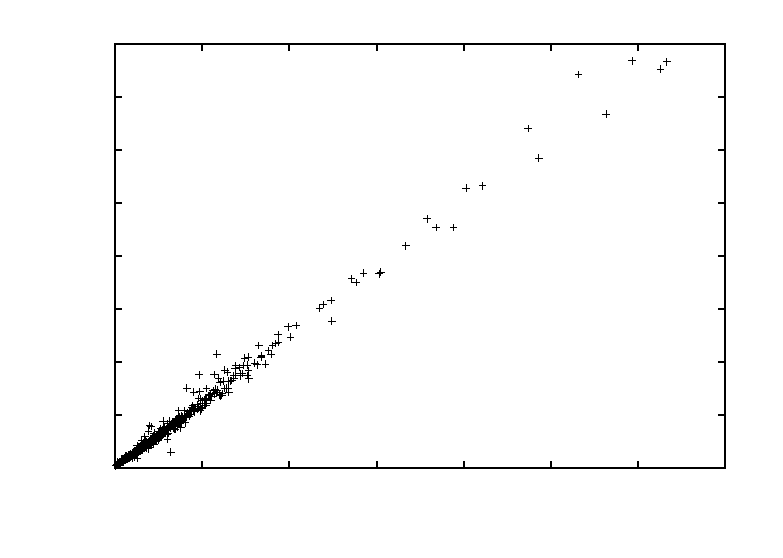
\includegraphics{plot}}%
    \gplfronttext
  \end{picture}%
\endgroup
%\end{document}

\end{frame}
%%%%%%%%%%%%%%%%%%%%%%%%%%%%%%%%%%%%%%%%%%%%%%%%%%%%%%%%%%%%%%%%%%%%%%%%%%%%%%%%
\section{Future works}
\begin{frame}{Works in next week}
\transwipe[direction=270]
\begin{itemize}[<+->]
\item Implementing \alert{Longest Common Substring} algorithm using
\alert{Generalised Suffix Tree} based on Ukk's algorithm.
\item Implementing \alert{Tokenization} on Python codes.
\item Implementing \alert{DC3} algorithm of \alert{Suffix Array} and compare
their performance.
\item Reading and Understanding \alert{n-gram} algorithm and its
application in code-clone detectation.
\end{itemize}
\end{frame}
\end{document}
